%% genome_features.tex
%% Author: Leighton Pritchard
%% Copyright: James Hutton Institute
%% Genome features

%
\begin{frame}
  \frametitle{Gene features}
  \textcolor{hutton_green}{Genes:}
  \begin{columns}[T] 
    \column{.4\textwidth} 
      \begin{itemize}
        \item translation start
        \item introns
        \item exons
        \item translation stop
        \item translation terminator
      \end{itemize}
    \column{.6\textwidth}
      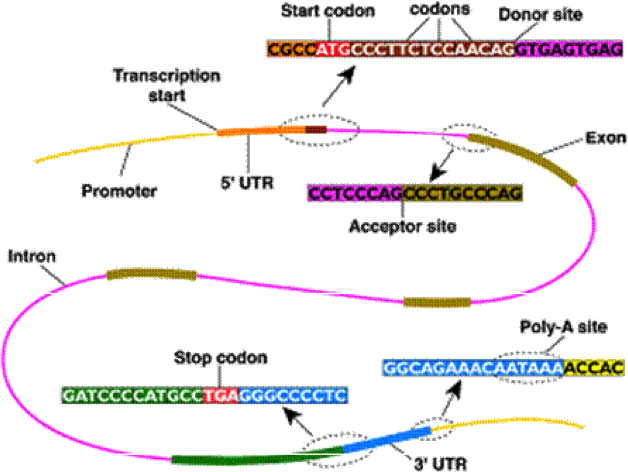
\includegraphics[width=\textwidth]{images/gene_feature}
  \end{columns}    
\end{frame}

%
\begin{frame}
  \frametitle{RNA features}
  \textcolor{hutton_blue}{RNA/ncRNA: characterised by complex secondary structure}
  \begin{columns}[T] 
    \column{.4\textwidth} 
      \begin{itemize}
        \item tRNA - transfer RNA
        \item rRNA - ribosomal RNA
        \item CRISPRs - prokaryotic defence, and genome editing
        \item many other functional classes, including enhancers
      \end{itemize}
    \column{.6\textwidth}
      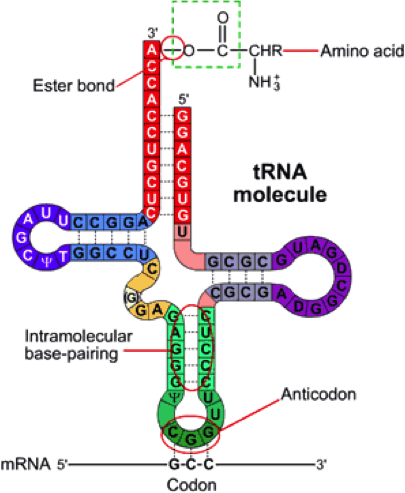
\includegraphics[height=0.7\textheight]{images/rna_feature}
  \end{columns}    
\end{frame}

%
\begin{frame}
  \frametitle{Gene features}
  \textcolor{hutton_green}{Regulatory sites:}
  \begin{itemize}
    \item transcription start sites (TSS)
    \item RNA polymerase (RNAp) binding sites
    \item transcription factor binding sites (TFBS)
    \item core, proximal and distal promoter regions
  \end{itemize}
  	
  \includegraphics[width=\textwidth]{images/_feature}
  \end{columns}    
\end{frame}

%
\begin{frame}
  \frametitle{Gene features}
  \textcolor{hutton_blue}{Genes:}
  \begin{columns}[T] 
    \column{.4\textwidth} 
      \begin{itemize}
        \item translation start
        \item introns
        \item exons
        \item translation stop
        \item translation terminator
      \end{itemize}
    \column{.6\textwidth}
      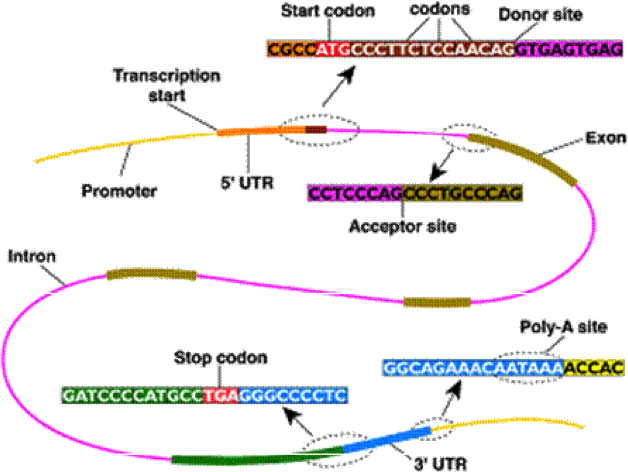
\includegraphics[width=\textwidth]{images/gene_feature}
  \end{columns}    
\end{frame}